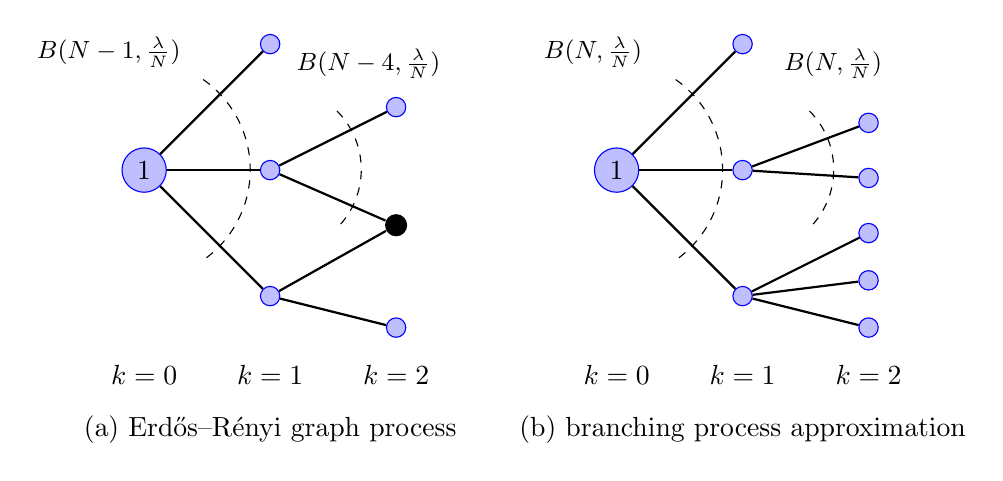
\begin{tikzpicture}[
  v/.style={circle, draw=blue, fill=blue!25, minimum size=7pt, inner sep=0pt},
  root/.style={circle, draw=blue, fill=blue!25, minimum size=16pt, inner sep=0pt},
  e/.style={thick}]
% (a) Erdos-Renyi graph process
\begin{scope}
  \node[root] (r) at (0,0) {$1$};
  \node[v] (a) at (1.6,1.6) {};
  \node[v] (b) at (1.6,0) {};
  \node[v] (c) at (1.6,-1.6) {};
  \node[v] (b1) at (3.2,0.8) {};
  \node[circle, fill=black, minimum size=8pt, inner sep=0pt] (s) at (3.2,-0.7) {};
  \node[v] (c2) at (3.2,-2.0) {};
  \draw[e] (r) -- (a); \draw[e] (r) -- (b); \draw[e] (r) -- (c);
  \draw[e] (b) -- (b1); \draw[e] (b) -- (s); \draw[e] (c) -- (s); \draw[e] (c) -- (c2);
  \draw[dashed] (0.75,1.15) arc (55:-55:1.4);
  \draw[dashed] (2.45,0.75) arc (45:-45:1.05);
  \node[font=\small] at (-0.45,1.5) {$B(N-1,\frac{\lambda}{N})$};
  \node[font=\small] at (2.85,1.35) {$B(N-4,\frac{\lambda}{N})$};
  \node at (0,-2.6) {$k=0$}; \node at (1.6,-2.6) {$k=1$}; \node at (3.2,-2.6) {$k=2$};
  \node at (1.6,-3.3) {(a) Erd\H{o}s--R\'enyi graph process};
\end{scope}
% (b) branching process approximation
\begin{scope}[xshift=6cm]
  \node[root] (r) at (0,0) {$1$};
  \node[v] (a) at (1.6,1.6) {};
  \node[v] (b) at (1.6,0) {};
  \node[v] (c) at (1.6,-1.6) {};
  \node[v] (b1) at (3.2,0.6) {};
  \node[v] (b2) at (3.2,-0.1) {};
  \node[v] (c1) at (3.2,-0.8) {};
  \node[v] (c2) at (3.2,-1.4) {};
  \node[v] (c3) at (3.2,-2.0) {};
  \draw[e] (r) -- (a); \draw[e] (r) -- (b); \draw[e] (r) -- (c);
  \draw[e] (b) -- (b1); \draw[e] (b) -- (b2);
  \draw[e] (c) -- (c1); \draw[e] (c) -- (c2); \draw[e] (c) -- (c3);
  \draw[dashed] (0.75,1.15) arc (55:-55:1.4);
  \draw[dashed] (2.45,0.75) arc (45:-45:1.05);
  \node[font=\small] at (-0.3,1.5) {$B(N,\frac{\lambda}{N})$};
  \node[font=\small] at (2.75,1.35) {$B(N,\frac{\lambda}{N})$};
  \node at (0,-2.6) {$k=0$}; \node at (1.6,-2.6) {$k=1$}; \node at (3.2,-2.6) {$k=2$};
  \node at (1.6,-3.3) {(b) branching process approximation};
\end{scope}
\end{tikzpicture}
